\subsection{Przybliżenie równania Laplace'a układem równań różnicowych}

% Pierwszy link odnosi się do pliku na komputerze autora oryginalnego PDFa lub do lokalizacji na serwerze Bubaka, do której nie mamy dostępu (w co wątpię).
% Drugi link jest martwy, odpowiedni wydział odpowiedniej uczelni ma już nową stronę internetową, na której nie znalazłem podanych treści.

\begin{frame}{\large{Przybliżenie równania Laplace'a układem równań różnicowych}}
  \centerline{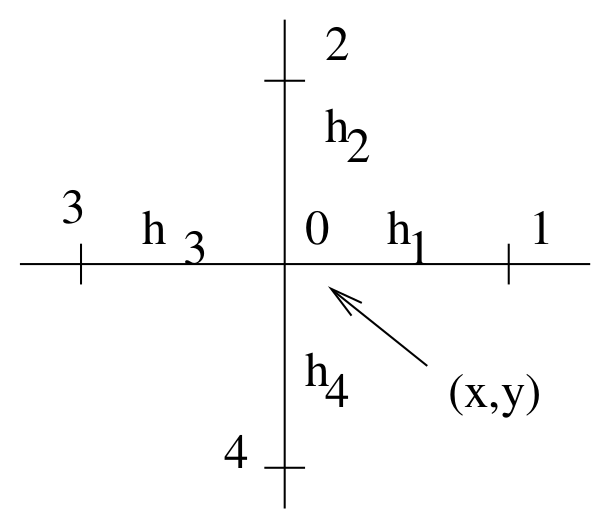
\includegraphics[width = 0.5 \linewidth]{img/23/przyblizanie}}
  $h>0, \qquad 0<h_i \le h, \qquad i = 1,2,3,4$ \\
  $u_i$  -- $u$ w punkcie $i$
\end{frame}

\begin{frame}
  Wyznaczamy parametry $\alpha_i$, $i=0, \dots ,4$ takie, by w $(x,y)$:
\begin{equation} \label{2}
\begin{split}
  u_{xx} + u_{yy} \equiv \alpha_0 \cdot u_0 + \alpha_1 \cdot u_1 + \alpha_2 \cdot u_2 + \alpha_3 \cdot u_3 + \alpha_4 \cdot u_4
\end{split}
\end{equation}

  Do $(\ref{2})$ podstawiamy rozwinięcia $u$ w szereg Taylora wokół $(x,y)$:
  $$ \begin{array}{l}
    u_1 = u_0 + u_x \cdot h_1 + \frac{1}{2} u_{x x} h_1^2 + O(h_1^3) \\
    u_2 = \ldots
  \end{array} $$

  Wtedy:
\begin{equation}
\begin{split}
u_{x x} + u_{y y} \equiv u_0 \cdot (\alpha_0 + \alpha_1 + \alpha_2 + \alpha_3 + \alpha_4) + u_x \cdot (h_1 \alpha_1 - h_3 \alpha_3) + \\
    + u_y \cdot (\alpha_2 h_2 - \alpha_4 h_4) + \frac{1}{2} u_{x x} \cdot (h_1^2 \alpha_1 + h_3^2 \alpha_3) + \\
    + \frac{1}{2} u_{y y} \cdot (h_2^2 \alpha_2 + h_4^2 \alpha_4) + \sum_{i=1}^4 O(h_i^3)
\end{split}
\end{equation}
\end{frame}

\begin{frame}
  Porównując ze sobą odpowiednie współczynniki, a następnie rozwiązując układ pięciu równań, mamy:
  \begin{block}{}
    $$ \begin{array}{l}
    \alpha_0 = -2 \cdot \left[ \frac{1}{h_1 h_3} + \frac{1}{h_2 h_4} \right], \\
    \alpha_1 = \frac{2}{h_1 (h_1 + h_3)}, \\
    \alpha_2 = \frac{2}{h_2 (h_2 + h_3)}, \\
    \alpha_3 = \frac{2}{h_3 (h_1 + h_3)}, \\
    \alpha_4 = \frac{2}{h_4 (h_2 + h_4)}
    \end{array}$$
  \end{block}

  Zastąpienie równania Laplace'a przybliżeniem $(\ref{2})$ opiera się na:
  $$ \lim_{h \rightarrow 0} \sum_{i=1}^4 [O(h_i^3)] = 0$$
\end{frame}

\begin{frame}
  Dla szczególnego, ważnego, przypadku:
  $$ h_1 = h_2 = h_3 = h_4 = h $$

  mamy:

  \begin{equation} \label{3} -4 u_0 + u_1 + u_2 + u_3 + u_4 = 0 \end{equation}

  z $(\ref{3})$ widać własność min-max:
  $$ u_0 = \frac{1}{4} (u_1 + u_2 + u_3 + u_4) $$

  czyli:
  \begin{block}{}
    $$ \min[u_1, u_2, u_3, u_4] \le u_0 \le \max[u_1, u_2, u_3, u_4] $$
  \end{block}

  Przedstawiony sposób transformacji PDE na równania różnicowe -- \textbf{uniwersalny}.
\end{frame}
